%%%%%%%%%%%%%%%%%%%%%%%%%%%%%%%%%%%%%%%%%
% Thin Sectioned Essay
% LaTeX Template
% Version 1.0 (3/8/13)
%
% This template is based on a downloaded from:
% http://www.LaTeXTemplates.com
%
% Original Author:
% Nicolas Diaz (nsdiaz@uc.cl) with extensive modifications by:
% Vel (vel@latextemplates.com)
% and adjustments by 
% Thuy Tran 
%
% License:
% CC BY-NC-SA 3.0 (http://creativecommons.org/licenses/by-nc-sa/3.0/)
%
%%%%%%%%%%%%%%%%%%%%%%%%%%%%%%%%%%%%%%%%%

%----------------------------------------------------------------------------------------
%	PACKAGES AND OTHER DOCUMENT CONFIGURATIONS
%----------------------------------------------------------------------------------------

\documentclass[a4paper, 12pt]{report} % Font size (can be 10pt, 11pt or 12pt) and paper size (remove a4paper for US letter paper)

\usepackage[protrusion=true,expansion=true]{microtype} % Better typography
\usepackage{graphicx} % Required for including pictures
\usepackage{wrapfig} % Allows in-line images
\usepackage{listings}
\usepackage{mathpazo} % Use the Palatino font
\usepackage[T1]{fontenc} % Required for accented characters
\usepackage[utf8]{inputenc} 
\usepackage[ngerman]{babel}
\linespread{1.05} % Change line spacing here, Palatino benefits from a slight increase by default
\usepackage{hyperref} %To include URLs

\makeatletter
\renewcommand\@biblabel[1]{\textbf{#1.}} % Change the square brackets for each bibliography item from '[1]' to '1.'
\renewcommand{\@listI}{\itemsep=0pt} % Reduce the space between items in the itemize and enumerate environments and the bibliography

\renewcommand{\maketitle}{ % Customize the title - do not edit title and author name here, see the TITLE block below
\begin{flushright} % Right align
{\LARGE\@title} % Increase the font size of the title

\vspace{50pt} % Some vertical space between the title and author name

{\large\@author} % Author name
\\\@date % Date

\vspace{40pt} % Some vertical space between the author block and abstract
\end{flushright}
}

%----------------------------------------------------------------------------------------
%	TITLE
%----------------------------------------------------------------------------------------

\title{\textbf{}\\ % Title
Terminal zur Bearbeitung von ARX-Daten mit R} % Subtitle

\author{\textsc{Alexander Beischl und Thuy Tran} % Author
\\{\textit{Technische Universität München}}} % Institution

\date{\today} % Date

%----------------------------------------------------------------------------------------

\begin{document}

\maketitle % Print the title section

%----------------------------------------------------------------------------------------
%	ABSTRACT AND KEYWORDS
%----------------------------------------------------------------------------------------

\renewcommand{\abstractname}{Zusammenfassung} % Uncomment to change the name of the abstract to something else

\begin{abstract}

Im Rahmen des Klinisches Anwendungsprojektes wurde die Java-Software \textit{R-Terminal} implementiert. Dieses Programm integriert die Programmiersprache und Entwicklungsumgebung \textit{R} in Java, sodass in der graphischen Benutzeroberfläche des \textit{R-Terminals} Befehle und Code eingegeben werden können, welche von \textit{R} ausgeführt werden. 

\end{abstract}


\vspace{30pt} % Some vertical space between the abstract and first section
%----------------------------------------------------------------------------------------

\tableofcontents


%----------------------------------------------------------------------------------------
%	ESSAY BODY
%----------------------------------------------------------------------------------------

\chapter{Einführung}\label{einführung}

This statement requires citation \cite{latexcompanion}; this one does too \cite{einstein}. Lorem ipsum dolor sit amet, consectetur adipiscing elit. Aenean dictum lacus sem, ut varius ante dignissim ac. Sed a mi quis lectus feugiat aliquam. Nunc sed vulputate velit. Sed commodo metus vel felis semper, quis rutrum odio vulputate. Donec a elit porttitor, facilisis nisl sit amet, dignissim arcu. Vivamus accumsan pellentesque nulla at euismod. Duis porta rutrum sem, eu facilisis mi varius sed. Suspendisse potenti. Mauris rhoncus neque nisi, ut laoreet augue pretium luctus. Vestibulum sit amet luctus sem, luctus ultrices leo. Aenean vitae sem leo.

Nullam semper quam at ante convallis posuere. Ut faucibus tellus ac massa luctus consectetur. Nulla pellentesque tortor et aliquam vehicula. Maecenas imperdiet euismod enim ut pharetra. Suspendisse pulvinar sapien vitae placerat pellentesque. Nulla facilisi. Aenean vitae nunc venenatis, vehicula neque in, congue ligula.

TODO Fabian bzgl. Lizenzen fragen

%------------------------------------------------

\section*{R}\label{r}
R ist eine Programmiersprache und Entwicklungsumgebung, die für statistische Berechnungen und Graphen unter John Chambers von Bell Laboratories entwickelt wurde. Sie ist ein GNU-Projekt, bei dem die Entwicklung von freier Software im Mittelpunkt steht. R weist große Ähnlichkeiten zu der Programmiersprache S auf, ein weiteres GNU-Projekt, welches weitgehend auch unter R läuft. \cite{rproject}

R bietet standardmäßig alle Hauptfunktionen an für die statistische Analyse von Datensätzen an und ist einfach zu erweitern, weswegen es vor allem für wissenschaftliche Arbeiten verwendet wird. Es ist mit R einfach, statistische Funktionen auf große Datenmengen anzuwenden.  


%------------------------------------------------

\section*{ARX}
ARX ist eine freie Software zur Anonymisierung von medizinischen Datensätzen, die von Fabian Prasser und Florian Kohlmayer vom Institut für medizinische Statistik und Epidemiologie an der Technischen Universität München entwickelt wurde.

\section*{Vorgaben}

Für die Implementierung der Software wurde Java als Programmiersprache vorgegeben, außerdem sollte die graphische Benutzeroberfläche mit \textit{SWT} realisiert werden.

Die graphische Benutzeroberfläche sollte aus unterschiedlichen Tabs aufgebaut sein. Ein Tab beinhaltet folgende Informationen zum Setup: verwendetes Betriebssystem, aktuell integrierte Version von \textit{R} und Installationsort der \textit{R}-Version. In einem weiteren Tab wird der Std-Output von \textit{R} ausgegeben und \textit{R}-Befehle können in diesen Tab eingegeben werden. 

Beim Programmstart soll automatisch in den Standart-Installationsorten nach einer ausführbaren \textit{R}-Executive gesucht werden. Außerdem soll die Möglichkeit bestehen, manuell eine \textit{R}-Installation auszuwählen und diese mit der Software in Java zu integrieren. 


\chapter{Anwenderdokumentation}
\section{Übersicht}
Das R-Terminal dient dazu, über eine externe Schnittstelle R aufzurufen und zu bedienen. Dies soll vor allem dazu genutzt werden, um Tabellen aus ARX einzuladen und Skripte auszuführen, und gleichzeitig die im Kapitel \ref{einführung} beschriebenen Probleme zu umgehen. Das R-Terminal ist kompatibel mit Windows, der Linux Distribution Ubuntu und OS X, von denen jeweils die folgenden Versionen im Rahmen der Entwicklung getestet wurden: 

\begin{itemize}
\item Windows 10 Education (Version 1511)
\item OS X El Capitan (Version 10.11.1)
\item macOS Sierra (Version 10.12.2)
\item Ubuntu
\end{itemize}

%insert screenshot for linux and the correct ubuntu/opensuse version

In den folgenden Abschnitten werden die Grundfunktionen und zusätzliche Features des R-Terminals beschrieben. 

\section{Vorbereitungen}

\textbf{TODO} Installation von R im Vorhinein und Auswahl der richtigen SWT-Libraries beschreiben. (Auswahl der Libraries wird in \ref{swt}
 beschrieben ;)
 
\section{}

\begin{figure}[htpb]
\centering
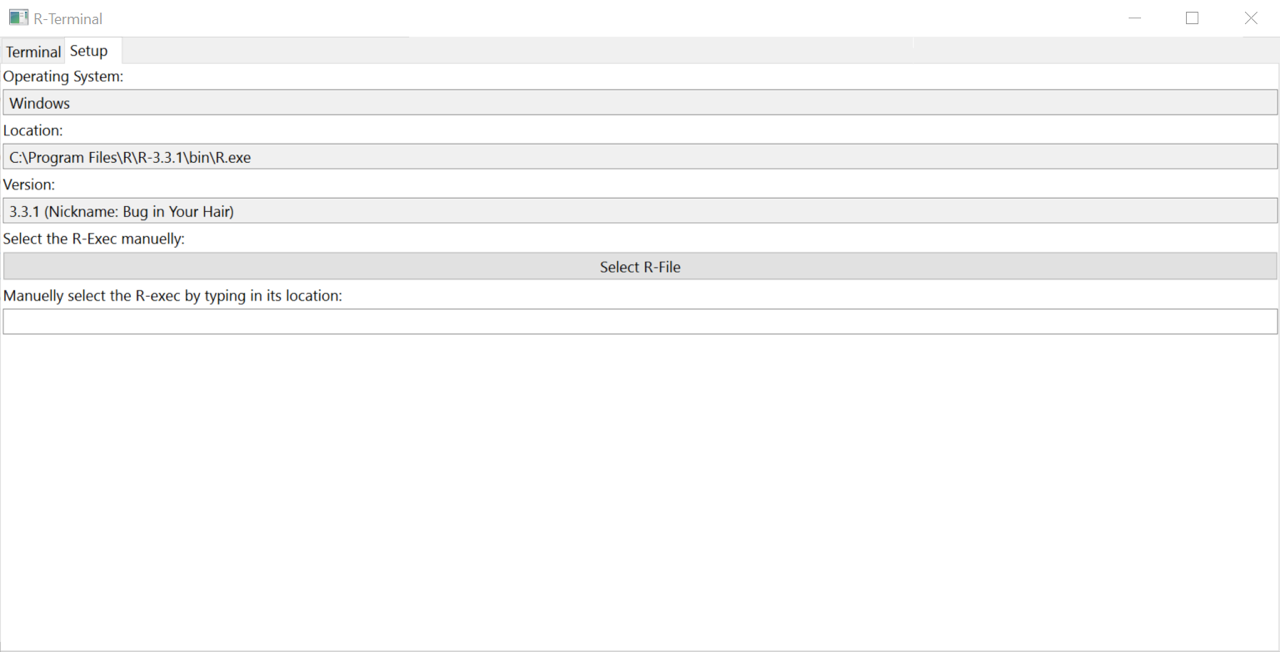
\includegraphics[width=0.8\textwidth]{R-TerminalWindows}
\caption{R-Terminal: \textit{Terminal} unter Windows 10 Education (Version 1511)}
\label{rterminalwindows}
\end{figure}

\begin{figure}[htpb]
\centering
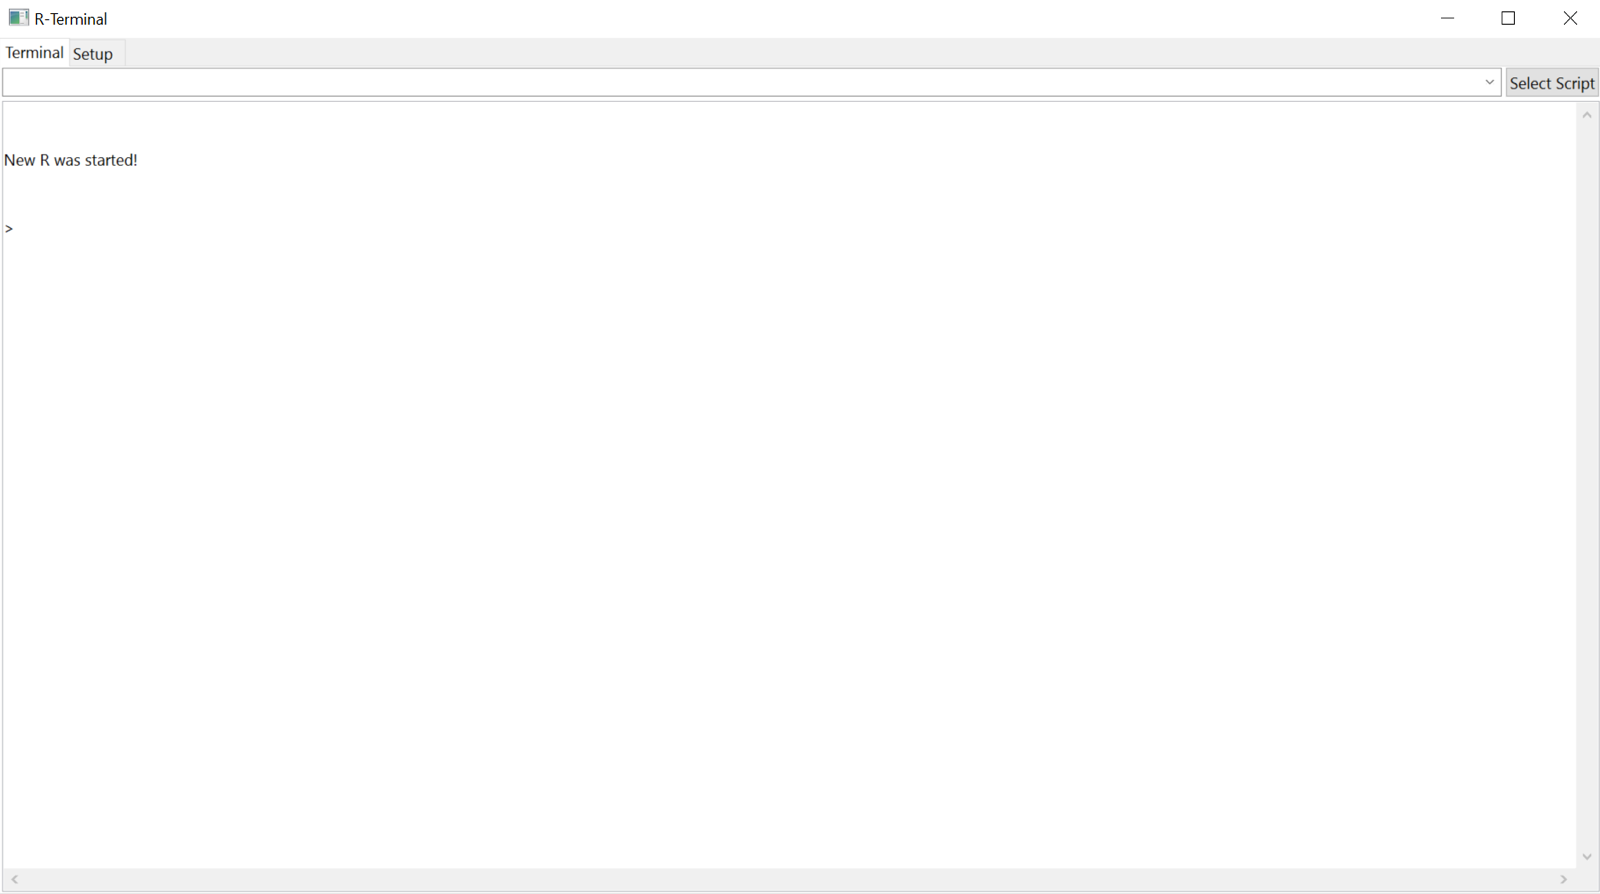
\includegraphics[width=0.8\textwidth]{rterminalwindows}
\caption{R-Terminal: \textit{Setup} unter Windows 10 Education (Version 1511)}
\label{rterminalwindows}
\end{figure}

\begin{figure}[htpb]
\centering
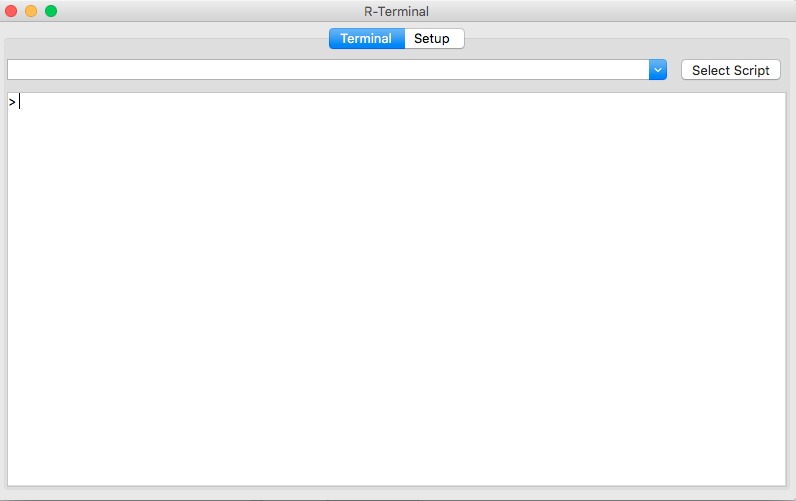
\includegraphics[width=0.8\textwidth]{R-Terminal}
\caption{R-Terminal: \textit{Terminal} unter OS X (Version 10.11.1)}
\label{rterminalmac}
\end{figure}

\begin{figure}[htpb]
\centering
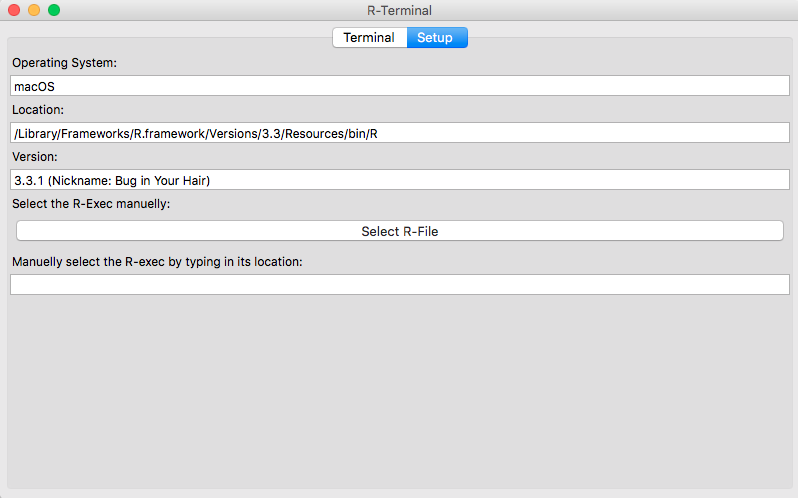
\includegraphics[width=0.8\textwidth]{rterminalsetup}
\caption{R-Terminal: \textit{Setup} unter OS X (Version 10.11.1)}
\label{macsetup}
\end{figure}

In Abbildung \ref{rterminalmac} ist das R-Terminal unter OS X (hier Version 10.11.1) zu sehen. Das Terminal verfügt über die beiden Tabs \textit{Terminal} und \textit{Setup} (s. \ref{macsetup)}. 

\subsection{Setup}
Unter \textit{Setup} wird entweder eine R-Version auf dem Rechner gesucht und automatisch ausgeführt oder es wird vom Benutzer selber der Pfad zu der gewünschten R-Version angegeben. 

Hierbei gibt das Feld unter \textit{Operating System} das Betriebssystem der benutzten Plattform an. Das Feld \textit{Location} gibt den Pfad an, unter dem die automatische Suche die ausführbare R-Version gefunden hat. Konnte keine ausführbare R-Version gefunden werden, wird in dem Feld die Nachricht \textit{No valid R-exec found!} angezeigt. 

Das mit \textit{Version} betitelte Feld gibt die Version an, die die gefundene R-Version hat. Wurde keine ausführbare R-Version gefunden oder eine ungültige R-Version angegeben, zeigt das Feld die Ausgabe \textit{No valid R-Version selected}an. 

Sind auf dem Rechner mehrere R-Versionen vorhanden, von denen der Benutzer eine andere Version bevorzugt, als die durch die manuelle Suche gefundene, gibt es die beiden unteren, im folgenden erläuterten Felder als Optionen. 

\textit{Select the R-Exec manually} öffnet eine Ordnerübersicht, durch die dann die zu der gewünschten R-Version navigiert werden kann. Hierbei sollte beachtet werden, dass nicht der Pfad zu der R-GUI angegeben werden sollte, welche oft zusammen mit dem R-Executable installiert wird, sondern zu der ausführbaren R-Datei.
  
Das letzte Feld \textit{Manually select the R-exec by typing in its location} gibt dem Benutzer die Möglichkeit, den bereits bekannten Dateipfad zur ausführbaren R-Datei anzugeben. Hierbei sollte ein absoluter Dateipfad angegeben werden, der die ausführbare R-Datei enthält (im Gegensatz dazu, nur den Ordner anzugeben, in dem die Datei liegt). 

Wird in \textit{Select the R-Exec manually} oder in \textit{Manually select the R-exec by typing in its location} eine ungültige R Version oder ein ungültiger Dateipfad angegeben, wird unter \textit{Operating System} und \textit{Version} dieselbe Fehlermeldung angegeben, wie oben bei dem Fehlschlagen der automatischen Suche beschrieben.

\subsection{Terminal}
Nachdem die gewünschte R-Version gefunden wurde, kann diese nun unter dem Tab \textit{Terminal} bedient werden. Das Eingabefeld kann benutzt werden, um R-kompatible Befehle auszuführen. Es werden bis zu 10 Befehle gespeichert. Diese können ausgewählt werden, indem auf den Pfeil auf der rechten Seite des Eingabefeldes geklickt wird. Dadurch öffnet sich ein Dropdown-Menü, aus dem der gewünschte Befehl ausgewählt werden kann. Dieser erscheint im Eingabefeld. 


\section{Benutzung von R für ARX }
Dieser Abschnitt wird sich mit der Benutzung von R im Zusammenhang mit großen Datentabellen befassen, wie sie in ARX üblich sind. Dies soll die Benutzung von dem R-Terminal zur Verarbeitung von ARX-Daten ermöglichen. 


\subsection{Skalenniveau}
In der medizinischen Statistik ist die Unterscheidung von den verschiedenen Stufen der Skalierbarkeit von großer Bedeutung. Für die Daten aus ARX sind vor allem die Eigenschaften wichtig, die Patientenmerkmale besitzen. So können Merkmale in quantitative und qualitative Merkmale unterteilt werden \cite{skalenniveau}. Es ist kein Problem, quantitative Merkmale darzustellen, da diese einfach durch numerische Werte ausgedrückt werden können. Die Grunddatentypen sind wie folgt:

\begin{itemize}
\item Numeric
\item Integer
\item Complex
\item Logic
\item Character
\end{itemize}

Wenn also eine Variable als Dezimalzahl ohne zusätzliche Bedingung deklariert wird, ist der Datentyp standardmäßig \texttt{numeric} (vgl. \ref{numericVar}).

\lstset{language=R}
\begin{lstlisting}[frame=single, caption = Deklarierung einer numerischen Variable x]
x = 13.4
\end{lstlisting}
\label{numericVar}

Will man explizit einen Integer als Variable initialisieren, sieht der Befehl aus wie in \ref{integerVar}.

\lstset{language=R}
\begin{lstlisting}[frame=single, caption = Deklarierung einer numerischen Variable x]
x = 13.4
\end{lstlisting}
\label{numericVar}


%insert skalenniveau Erklärung 
%insert data.frame erklärung
%insert rbind und cbind
%insert Erklärung zu data.table und data.matrix 


\newpage

\chapter{Entwicklerdokumentation}

\section{Verwendete Technologien}

Das \textit{R-Terminal} wurde mit der Entwicklungsumgebung \textit{Eclipse} entwickelt.
Als Programmiersprache wurde \textit{Java} gewählt. Die graphische Benutzeroberfläche wurde mit \textit{SWT} realisiert, genauere Details hierzu werden in \ref{swt} erläutert.
Um \textit{R}-Kommandos auszuführen, startet das hier dokumentierte Programm \textit{R-Terminal} einen \textit{R}-Prozess der Standalone-Installation von \textit{R} durch die Java-Library \textit{ProcessBuilder}.


\section{Architektur des R-Terminals}

Die Software des \textit{R-Terminal} ist in zwei Komponenten aufgeteilt, welche als getrennte Packages vorliegen. Das erste Package "`org.deidentifier.arx.gui"' beinhaltet die graphische Benutzeroberfläche, das Zweite "`org.deidentifier.arx.r"' beinhaltet die gesamte Integration von \textit{R} in \textit{Java}, es stellt also alle funktionalen Methoden zur Verfügung und verwaltet die Kommunikation zwischen \textit{R} und dem \textit{Java}-Programm.

Durch die Trennung von graphischer Benutzeroberfläche und der Integration von \textit{R}, also dem funktionalen Kern, kann die \textit{R}-Integration auch ohne graphische Benutzeroberfläche ausgeführt und verwendet werden. Hierzu wird nur das zweite Package benötigt, welches in \ref{funktionaler Kern} behandelt wird. Die Ausführung ohne GUI wird in \ref{ohne GUI} erläutert.\\

Alle Klassen der Software \textit{R-Terminal}, sowie deren wichtigsten Methoden, werden in den Kapiteln \ref{gui} und \ref{funktionaler Kern} vorgestellt.

\section{Graphische Benutzeroberfläche (GUI)}\label{gui}

\begin{samepage}

Das erste Package, "`org.deidentifier.arx.gui"', erzeugt und verwaltet die graphische Benutzeroberfläche. Es umfasst sieben Klassen:
\begin{itemize}
	\item RMain
	\item RTerminal
	\item RSetupTab
	\item RTerminalTab
	\item RBrowserWindow
	\item RLayout
	\item RCommandListener
\end{itemize}
\end{samepage}

\subsection{RMain}

Um das Programm mit einer graphischen Benutzeroberfläche zu starten, muss die "`main"'-Methode der Klasse \textit{RMain} ausgeführt werden. 

Diese erzeugt ein neues Display sowie eine Shell. Im Anschluss wird ein neues Objekt der Klasse \textit{RTerminal} erzeugt.

\subsection{RTerminal}

Die Erzeugung der einzelnen Komponenten der graphischen Benutzeroberfläche wird durch den Konstruktor der Klasse \textit{RTerminal} realisiert.

Dieser erzeugt einen TabFolder mit zwei Tabs, der erste Tab beinhaltet ein Objekt der Klasse \textit{RTerminalTab}, der zweite ein Objekt der Klasse \textit{RSetupTab}.
Außerdem erzeugt der Konstruktor noch einen Ring-Puffer "`buffer"', welcher zur Speicherung des Std-Output von \textit{R} verwendet wird, sowie einen Listener "`listener"'. Sowohl der Ring-Puffer, als auch der Listener wurden im Package "`org.deidentifier.arx.r"' implementiert.
Im Anschluss wird die Integration mit \textit{R} durch den Aufruf der Methode "`startRIntergration"' eingeleitet.\\

Diese Methode "`startRIntergration"' erzeugt ein neues Objekt der Klasse "`RIntegration"', welches in \ref{RIntegration} beschrieben wird und die Integration von \textit{R} realisiert.
\\

TODO Listener Methodenüberschreiben

\subsection{RSetupTab}

Die Klasse \textit{RSetupTab} erzeugt einen Tab, welcher Informationen zum verwendeten Betriebssystem sowie dem aktuellen Status der Integration von \textit{R} anzeigt.\\

Die unterschiedlichen Informationen werden in \textit{SWT}-Labels dargestellt, welche in einem \textit{GridLayout} angeordnet sind.
Die \textit{SWT}-Labels werden durch die Methodenaufrufe "`showOS()"', "`showRLocation()"', "`showRVersion()"' im Konstruktor erzeugt.

Um das verwendete Betriebssystem abzufragen, wird die Methode "`printOS()"' der Klasse \textit{OS}, siehe \ref{OS}, von "`showOS()"' aufgerufen. Diese gibt das verwendete Betriebssystem als String zurück.

%Das aktuell verwendete Betriebssystem wird durch den Aufruf der Methode "`printOS()"' der Klasse \textit{OS} aus dem zweiten Package aufgerufen. Weitere Informationen hierzu finden sich in \ref{OS}.

Die Integration von \textit{R} wird in der Klasse \textit{RIntegration} des  Package "`org.deidentifier.arx.r"' umgesetzt. Diese wird beim Start des Programms in \textit{RTerminal} aufgerufen. 
 Um den Status der Integration zu prüfen, rufen "`showRLocation()"' und "`showRVersion()"' die Methode "`getR()"' aus \textit{OS} auf. Diese gibt den absoluten Pfad zur aktuell verwendeten R-Executive zurück, welcher im \textit{RSetupTab} angezeigt wird.
Wurde keine R-Executive gefunden oder konnte diese nicht erfolgreich gestartet werden, so wird von "`getR()"' \textit{null} zurückgegeben und im \textit{RSetupTab} wird ausgegeben:  
\begin{center}
Location: "`No falid R-exec found!"'

Version: "`No falid R-Version selected!"'
\end{center}

Wurde eine \textit{R}-Version gefunden und erfolgreich ausgeführt, so wird der erzeugte Listener in \textit{RTerminal} ausgelöst. Dieser ruft anschließend die Methode "`update()"' auf, durch welche der Inhalt von Location und Version aktualisiert wird.\\

Außerdem ermöglicht der \textit{RSetupTab} die manuelle Auswahl einer \textit{R}-Executive. Im Konstruktor wird hierfür ein Knopf mit "`createManuellSearchWindow()"' zum Öffnen eines Navigationsfensters sowie eine Kommandozeile "`createDirSearchLine()"' erzeugt, sodass entweder der absolute Pfad zur Datei angegeben oder diese mittels des Navigationsfensters ausgewählt werden kann.

Die Kommandoleiste wird in der Methode "`createDirSearchLine()"' erzeugt und erfasst die Eingabe durch einen \textit{TraverseListener}. Der \textit{TraverseListener} wird durch Drücken der Return-Taste ausgelöst und gibt den eingegeben Pfad an die Methode "`updateSetup($String$ path)"' weiter. Wird die \textit{R}-Executive mit dem Navigationsfenster gesucht, so wird der absolute Pfad der ausgewählten Datei ebenfalls an "`updateSetup($String$ path)"' als Argument übergeben. Nähere Informationen zum Navigationsfenster finden sich in \ref{RBrowserWindow}.

Die Methode "`updateSetup($String$ path)"' startet eine neue Integration von \textit{R} durch den Aufruf der Methode "`startManuellRIntegration($String$ path)"' aus der Klasse \textit{RTerminal}. Nähere Details hierzu in \ref{RTerminal}. 

Falls die \textit{R}-Executive erfolgreich gestartet wurde, wird durch den \textit{RListener} (siehe oben) der Tab wieder aktualisiert. Andernfalls wird die selbe Ausgabe angezeigt, wie bei der automatischen Suche.

\subsection{RTerminalTab} \label{RTerminal}

Im \textit{RTerminalTab} werden \textit{R}-Befehls-Eingaben des Nutzers erfasst sowie der Std-Output von \textit{R} ausgegeben. Außerdem können mittels eines Knopfes fertige \textit{R}-Skripte geladen und ausgeführt werden. Der \textit{RTerminalTab} ist nur nutzbar, falls \textit{R} erfolgreich gestartet und integriert wurde.\\

Der Tab hat als Layout ebenso wie der \textit{RSetupTab} ein \textit{GridLayout}.
Dieses besteht aus einem \textit{Composite} und einem Textfeld.\\

Das Kompositum "`topline"' umfasst eine Kommandozeile, ein Dropdown-Menü um eingegebene Befehle erneut auszuführen sowie einen Knopf zum Aufrufen von \textit{R}-Skripten. Als Layout wurde ebenfalls \textit{GridLayout} gewählt, da es alle Komponenten möglichst kompakt darstellt.

Die Kommandozeile und das Dropdown-Menü "`input"' wurden mit der importierten Klasse \textit{swt.widget.Combo} erstellt. Die Kommandozeile erfasst die Eingaben des Nutzers beim Drücken der Enter-Taste durch einen \textit{TraverseListener}. Die Eingabe wird anschließend an die Methode "`command($String$ command)"' der Klasse  \textit{RCommandListener} übergeben, welche den Befehl an \textit{R} übergibt. Dies wird in \ref{RCommandListener} genauer beschrieben.

Die letzten 10 eingegebenen Befehle werden im Dropdown-Menü angezeigt. Die Befehle werden in einem Ring-Puffer mit 10 Elementen gespeichert, welcher als String Array implementiert wurde.\\

Skripte können durch den Knopf "`scriptButton"' ausgewählt und ausgeführt werden. Der Knopf wird durch einen \textit{MouseListener} ausgelöst und erzeugt ein Navigationsfensters der Klasse \textit{RBrowserWindow}. Weiter Informationen hierzu in \ref{RBrowserWindow}. Durch dieses kann das Skript ausgewählt werden und es wird vom \textit{RBrowserWindow} der absolute Pfad des Skriptes übergeben. Anschließend wird überprüft, ob es sich um ein \textit{R}-Skript handelt, also die Datei auf "`.r"' endet. Trifft dies zu, so wird durch die Methode "`command($String$ command)"' der Klasse  \textit{RCommandListener} der Befehl das Skript zu öffnen an \textit{R} übergeben. Dieser setzt sich zusammen aus:
\begin{center}
$source("$  absoluter Pfad $")$.	
\end{center}


Das Textfeld "`output"' beinhaltet die Ausgabe von \textit{R} und wurde durch die importierte Klasse \textit{StyledText} realisiert. Das Textfeld ist als Ring-Puffer implementiert, sodass dieser nur die letzten $10000$ Zeichen des \textit{R}-Std-Output anzeigt. Die Größe des Ring-Puffers ist in der Klasse \textit{RTerminal} als globale int Variable "`BUFFER\_SIZE"' festgelegt und kann hier geändert werden.
Der Std-Output von \textit{R} wird durch das Auslösen des RListener "`listener"' in \textit{RTerminal} aktualisiert. Dieser ruft hierzu die Methode "`setOutput($String$ text)"' aus \textit{RTerminalTab} auf. Der Listener wird nach erfolgreichem Starten von \textit{R} durch die Klasse \textit{RIntegration} übergeben. Diese ruft die Methode "`setCommandListener($RCommandListener$ listener)"' im \textit{RTerminalTab} auf und übergibt den Listener als Argument. Details zum Listener finden sich in \ref{RCommandListener}.\\

Außerdem wird nach einem erfolgreich Start von \textit{R} durch "`startRIntegration($String$ path)"' aus der Klasse \textit{RTerminal}  die Methode "`enableTab()"' in \textit{RTerminalTab} aufgerufen, sodass der Tab nutzbar wird. Beim Beenden von \textit{R} wird in der Methode "`endR()"' in  \textit{RTerminal} die Methode "`disableTab()"' in \textit{RTerminalTab} aufgerufen, welche den Tab wieder für den Nutzer sperrt.

\subsection{RBrowserWindow} \label{RBrowserWindow} 

Die Klasse \textit{RBrowserWindow} implementiert ein Navigationsfenster des Standart-Dateimanagers. 
Dieses wurde durch die importierte \textit{SWT}-Klasse \textit{FileDialog} implementiert. Die Klasse beinhaltet nur eine Methode "`openBrowser(Shell)"', durch welche ein neuer \textit{FileDialog}, also ein Navigationsfenster, erzeugt wird, mit welchem eine Datei ausgewählt werden kann. Anschließend gibt die Methode den absoluten Pfad der ausgewählten Datei zurück. 
Mit dem Navigationsfenster kann sowohl manuell die \textit{R}-Executive im \textit{RSetupTab} sowie ein ausführbares \textit{R}-Skript im \textit{RTerminalTab} ausgewählt werden. Anschließend wird der absolute Pfad per \textit{return} übergeben, sodass der funktionale Kern, siehe \ref{funktionaler Kern}, die jeweilige Aktion durchführen kann.

\subsection{RLayout}

Diese Klasse definiert das \textit{SWT}-Layout der Klassen \textit{RSetupTab} und \textit{RTerminalTab}. 
Die Methoden der Klasse werden im Konstruktur der beiden genannten Klassen aufgerufen, um die \textit{SWT}-Objekte der des jeweiligen Tabs mit den richtigen Parametern und Abständen zu erzeugen.

\subsection{RCommandListener} \label{RCommandListener}

Das Java-Interface \textit{RCommandListener} implementiert einen Listener, welcher bei der Eingabe von Befehlen für \textit{R} ausgeführt wird. Die abstrakte Methode "`command($String$ command)"' des Interfaces wird in der Klasse \textit{RTerminal} mit der Methode "`execute(command)"' aus der Klasse \textit{RIntegration} überschrieben. Somit wird die Trennung der graphischen Oberfläche und des funktionalen Kerns der \textit{R}-Integration, welcher in \ref{funktionaler Kern} beschrieben wird, beibehalten.


\section{Funktionaler Kern - Integration von R} \label{funktionaler Kern}

Die Integration von \textit{R} in Java ist in dem Package "`org.deidentifier.arx.r"' implementiert. Dieses beinhaltet alle Funktionen, durch welche die \textit{R}-Executive automatisch gefunden, ausgeführt und das Betriebssystem erkannt wird. Außerdem beinhaltet es alle Methoden zur Übermittlung des Input- und Outputstreams.
Zur Integration von \textit{R} in Java wurde die Klasse \textit{ProcessBuilder} verwendet.

\begin{samepage}
Das Package umfasst vier Klassen:
\begin{itemize}
	\item RIntegration
	\item OS
	\item RBuffer
	\item RListener
\end{itemize}
\end{samepage}


\subsection{RIntegration} \label{RIntegration}

Die Klasse \textit{RIntegration} ist das Kernstück des \textit{R-Terminals} und ist für die Integration von \textit{R} verantwortlich. Der \textit{R}-Prozess wird durch die Library \textit{ProcessBuilder} gestartet.

Wird das Programm mit der graphischen Benutzeroberfläche gestartet, so wird für jede gefundene ausführbare \textit{R}-Executive durch die Methode "`startRIntegration"' beziehungsweise "`startManuellRIntegration"' ein neues Objekt dieser Klasse erzeugt.
Hierbei werden dem Konstruktor folgende Argumente übergeben:
\begin{itemize}
	\item $final$ $String$ path
	\item $final$ $buffer$ buffer 
	\item $final$ $RListener$ listener
\end{itemize}
%
Der absolute Pfad zur Executive wird durch "`path"' angegeben. Bei "`buffer"' handelt es sich um den Ring-Puffer der Klasse \textit{RBuffer}, welcher zur Ausgabe des Std-Output des \textit{R}-Prozesses im \textit{RTerminalTab} erzeugt wurde. Gibt es eine neue Ausgabe des Std-Output des Prozesses, so wird dieser im Ring-Puffer angehängt. 
Um die beiden Tabs \textit{RSetupTab} und \textit{RTerminalTab} bei Änderungen zu aktualisieren, wird der \textit{RListener}, welcher in \textit{RTerminal} erzeugt wurde, als Attribut "`listener"' übergeben.
Bei einer Ausgabe des Std-Output oder Start bzw. Beenden des \textit{R}-Prozesses wird dieser ausgelöst.\\

Der Konstruktor erzeugt ein neues Objekt der Klasse \textit{ProzessBuilder} mit den betriebssystemspezifischen Parametern. Die Parameter werden durch Aufrufen der Methode "`getParameters($String$ path)"', siehe \ref{OS}, aus der Klasse \textit{OS} übergeben und dem Konstruktor des \textit{ProzessBuilders} als Argumente übergeben.

Anschließend wird der Prozess gestartet.\\

Nach erfolgreichen Start des \textit{R}-Prozesses wird ein Reader "`reader"' erzeugt, welchem die Ausgabe des \textit{R}-Prozesses übergeben wird. Dieser Reader übergibt die Ausgabe an den Ring-Puffer "`listener"'.

Direkt im Anschluss wird die Methode "`getVersion($Reader$ reader)"' aufgerufen. Durch diese wird abgefragt, welche Version von \textit{R} verwendet wird.
Die Ausgabe der Version wird durch das Kommando "`version"', welches an den laufenden \textit{R}-Prozess als Input durch den Methodenaufruf "`execute("version")"' übergeben wird, erreicht. Die Ausgabe dieses Kommandos soll nicht im Ausgabefenster der GUI, dem \textit{RTerminalTab}, angezeigt werden. Deshalb erzeugt die Methode "`getVersion(Reader reader)"' einen neuen, temporären Ring-Puffer, in welchem die Ausgabe für diesen Befehl gespeichert wird. 

Aus dem Ausgabe-String dieses "`version"'-Kommandos wird anschließend die genaue Version sowie der Nickname extrahiert und in der lokalen Variable "`version"' gespeichert. Im Anschluss wird der Rlistener  "`listener"' ausgelöst, welcher die Methode "`setupUpdate()"' ausführt. Diese Methode ruft die "`update"'-Methode im \textit{RSetupTab} auf und aktualisiert den Tab.\\

Nach Abschluss dieses Kommandos wird die gesamte Ausgabe in den Ring-Puffer "`buffer"' geschrieben und durch Auslösen des RListener "`listener"' in dem Ausgabefenster des \textit{RTerminalTabs} angezeigt.\\

Kommandos, welche in \textit{R} ausgeführt werden sollen, werden als String der Methode "`execute($String$ command) "' übergeben, welche diese an den \textit{R}-Prozess weiterleitet. Hier wird ein \textit{BufferedWriter}-Objekt erstellt. Mit der "`write(String command)"' Methode dieses Elementes wird das Kommando in dem \textit{BufferedWriter} geschrieben und anschließend mit "`newline()"' noch ein Zeilenumbruch im \textit{BufferedWriter} gespeichert. Um den Inhalt des \textit{BufferedWriter} an den \textit{R}-Prozess zu übergeben, diesen auszuführen und anschließend den \textit{BufferedWriter} zu leeren, wird zum Abschluss die Methode "`flush()"' aufgerufen.
Mit dieser Methode werden alle Kommandos an den \textit{R}-Prozess übergeben. Die "`execute($String$ command)"' Methode wird bei der Nutzung der GUI von der Methode "`command($String$ command)"' aufgerufen. Nähere Informationen zur Methode "`command($String$ command)"' finden sich in \ref{RCommandListener}.

\subsection{OS} \label{OS}

Die Klasse \textit{OS} implementiert folgende Funktionalitäten: Erkennung des verwendeten Betriebsystems, die Anpassung der Pfade der Standart-Speicherorte der \textit{R}-Executive je nach verwendeten Betriebssystem und die Überprüfung der übergebenen \textit{R}-Executives.\\

Um die drei unterstützten Betriebssysteme Windows, Mac und Unix effizient zu unterscheiden, werden diese als Enum Konstanten "`OSType"' erzeugt.\\

Die absoluten Pfade der Standart-Speicherorte der \textit{R}-Executive werden für jedes Betriebssystem in einem eigenen String Array gespeichert. Es ist wichtig hier zu beachten, dass Windows andere Separatoren verwendet als Linux und OS X.
Bei Windows müssen die einzelnen Verzeichnisse durch "`$\backslash \backslash$"' getrennt werden, bei beiden anderen Betriebssystemen durch "`/"'. 

Falls neue Standart-Speicherorte für die \textit{R}-Executive hinzugefügt werden sollen, kann das jeweilige Array einfach um den neuen Pfad erweitert werden. Beim Starten des \textit{R-Terminals} durch die graphische Benutzeroberfläche werden alle Pfade des Arrays nach einer ausführbaren \textit{R}-Executive durchsucht.Hierfür wird die Methode "`getR()"' aufgerufen, welche im Folgenden noch vorgestellt wird.\\

Außerdem werden die Dateinamen der \textit{R}-Executive für die unterschiedlichen Betriebssysteme in einem String-Array gespeichert, da sich diese je nach Betriebssystem unterscheiden. Außerdem wird das jeweilige Array benötigt, um bei der manuellen \textit{R}-Auswahl zu prüfen, ob es sich um eine gültige \textit{R}-Executive handelt. Dies wird in der Methode "`isRExec($String$ path)"' in Abhängigkeit vom verwendeten Betriebssystems überprüft.\\

Die Methode "`getOS()"' fragt den Namen des Betriebssystems ab und gibt dieses als Enum "`OSType"' passend zurück.\\

Wie bereits beschrieben, werden nach dem Start des Programms die Standart-Speicherorte nach einer ausführbaren R-Executive durchsucht. Ob an einem dieser Speicherorte eine Executive liegt, wird mit der Methode "`getPath($String[]$ locations, $String[]$ executables)"' überprüft. Außerdem wird versucht die Executive mit \textit{ProcessBuilder} zu starten, um zu prüfen, ob der Nutzer ausreichende Zugriffsberechtigungen besitzt.\\

Zusätzlich sind in der Klasse \textit{OS} die Parameter zur Ausführung der \textit{R}-Executive für den \textit{ProcessBuilder} gespeichert. Diese werden beim Aufruf der Methode "`getParameters($String$ path)"' mit dem Pfad "`path"' der Executive zu einem String-Array konkateniert und anschließend als String-Array zurückgegeben.

\subsection{RBuffer} \label{RBuffer}

Diese Klasse implementiert den Ring-Puffer, welcher für die Ausgabe des Std-Output von \textit{R} im Ausgabefenster des \textit{RTerminalTab} verwendet wird.
Die Größe des Ring-Puffers wird bei der Erzeugung dem Konstruktor übergeben und ist beim Starten des Programms mit graphischer Benutzeroberfläche in der Klasse \textit{RTerminal} in der Variable "`BUFFER\_SIZE"' festgelegt.

\subsection{RListener} \label{RListener}

Die Klasse \textit{RListener} implementiert einen Listener, welcher in den Klassen \textit{RTerminal}, siehe \ref{gui}, sowie \textit{RIntegration} verwendet wird. \\

Der Listener aktualisiert die Inhalte von \textit{RSetupTab} sowie \textit{RTerminalTab}. 
Durch die abstrakte Methode "`setupUpdate()"', welche in \textit{RTerminal} überschrieben wird, wird bei Änderung des Status von \textit{R}, also dem Beenden oder dem Starten eines neuen \textit{R}-Prozesses der \textit{RSetupTab} aktualisiert.
Durch "`bufferUpdate()"' wird das Ausgabefenster im \textit{RTerminalTab} aktualisiert. Diese abstrakte Methode wird ebenfalls in \textit{RTerminal} überschrieben.



\section{Ausführung ohne graphische Benutzeroberfläche} \label{ohne GUI}

Der funktionale Kern des \textit{R-Terminals} kann auch ohne die graphische Benutzeroberfläche ausgeführt werden. Hierfür müssen allerdings folgende Objekte erzeugt werden:
\begin{itemize}
	\item ein Ring-Puffer der Klasse \textit{RBuffer}, welcher den Input für \textit{R} beinhaltet
	\item ein weiterer Ring-Puffer der selben Klasse, welchen den Std-Output von \textit{R} übergeben wird
	\item ein Listener der Klasse \textit{RListener}, welcher durch den Std-Output ausgelöst wird
\end{itemize}
	
Anschließend müssen die abstrakten Methoden des \textit{RListeners} überschrieben werden:
	\begin{itemize}
		\item \textit{bufferUpdated()}
		\item \textit{closed()}
		\item \textit{setupUpdate()}
	\end{itemize}

Anschließend kann die Integration von \textit{R} gestartet werden. Hierfür muss ein neues \textit{RIntegration}-Objekt erzeugt werden.


Um dem \textit{R}-Prozess nun Befehle zu übergeben, muss lediglich die Methode "`execute"' des erzeugten \textit{RIntegration}-Objekt aufgerufen werden und das Kommando als String übergeben werden.\\
\\
Beispiel: Es wurde ein \textit{RIntegration}-Objekt \textit{rProcess} erzeugt und es soll "`1+2+3+4+5"' als Kommando übergeben werden, dann muss
	\begin{center}
		\textit{rProcess}.execute("`1+2+3+4+5"')
	\end{center} 
	ausgeführt werden. Die Ausgabe wird im Ring-Puffer gespeichert, welcher für den Std-Output erzeugt wurde.\\
\\
Ein Code-Beispiel hierzu befindet sich im Package "`ExampleWithoutGUI"'.

\section{Abhängigkeiten}

Das Projekt beinhaltet bereits alle benötigten Java-Libraries zur Ausführung der Software. 
Da die graphische Benutzeroberfläche mit \textit{SWT} realisiert wurde, müssen die \textit{SWT}-Libraries je nach Betriebssystem ausgewählt werden. Dies wird genauer unter \ref{swt} erläutert.\\

Für die Integration von \textit{R} in Java, welche durch das \textit{R-Terminal} umgesetzt wurde, muss eine Standalone-Installation von \textit{R} vorliegen. Nähre Details hierzu in \ref{r}.
 
\subsection{Java}

Die für das \textit{R-Terminal} verwendetet Programmiersprache ist Java. Für die Entwicklung und Tests wurde \textit{Java SE 8 (1.8.0\_91)} verwendet.
 
\subsection{R-Project} \label{r}

Um \textit{R} in Java zu integrieren muss eine Standalone-Installation von R, für welche der aktuellen Benutzer ausreichende Zugriffsrechte besitzt, vorhanden sein. 
Alle aktuellen \textit{R}-Versionen können von der Homepage des \textit{R}-Projects\footnote{\url{https://www.r-project.org}} heruntergeladen werden. 


\subsection{SWT}\label{swt} 
Die graphische Benutzeroberfläche wurde mithilfe des \textit{Standard Widget Toolkit} (\textit{SWT}) realisiert. \textit{SWT} ist ein "`open-source widget toolkit"' für Java mit Integration in die GUI des nativen Betriebssystems, sodass das Design der Benutzeroberfläche an das Design des Betriebssystems angepasst wird. 

Für das Projekt \textit{R-Terminal} wurde die \textit{SWT}-Version 4.2.1 verwendet.\\

Wie die betriebssystemspezifischen \textit{SWT}-Libraries auf den "`Build Path"' hinzugefügt werden, kann unter \ref{swtanwender} nachgeschlagen werden.\\
\\
\textbf{TODO vlt in die Anwenderdokumentation?}\\

\label{swtanwender}

Um das \textit{R-Terminal} ausführen zu können, müssen die betriebssystemspezifischen \textit{SWT}-Libraries auf den Bild-Path gesetzt und die \textit{SWT}-Libraries anderer Betriebssysteme entfernt werden.
Im Folgenden wird genau beschrieben, wie dies unter \textit{Eclipse} umgesetzt wird:
\begin{enumerate}
	\item Navigieren Sie im \textit{Eclipse} Package Explorer zu:
	\begin{center}\textit{R-Terminal -> lib  -> swt} \end{center}
	
	\item Wählen Sie die betriebssystemspezifischen \textit{SWT}-Libraries aus und öffnen Sie mit der rechten Maustaste, bzw. dem OS-spezifischen Äquivalent, für jede dieser Libraries das Auswahlfenster. Klicken Sie auf "`Build-Path"'.
		Sollte die Library bereits hinzugefügt sein, erscheint "`Configure Build Path..."'. Ist dies nicht der Fall, erscheint "`Add to Build Path"', klicken Sie dieses an.\\
		
	Betriebssystemspezifische \textit{SWT}-Libraries:
		
	\begin{itemize}
		\item Windows: \begin{itemize}
							\item swt-4.2.1-win32-win32-x86\_64.jar
							\item swt-4.2.1-win32-win32-x86.jar
						\end{itemize}
						
		\item Mac: \begin{itemize}
						\item swt-4.2.1-cocoa-macosx-x86\_64.jar
						\item swt-4.2.1-cocoa-macosx.jar
					\end{itemize}
		\item Linux: \begin{itemize}
						\item swt-4.2.1-gtk-linux-x86\_64.jar
						\item swt-4.2.1-gtk-linux-x86.jar
					 \end{itemize}
	\end{itemize} 
	
	\item Überprüfen Sie nun, ob alle anderen Libraries des Ordners \textit{swt} nicht auf dem "`Build Path"' liegen. 
		Gehen Sie hierfür zu:
		\begin{center}
			\textit{R-Terminal -> Referenced Libraries}
		\end{center} 
		
		Überprüfen Sie, dass keine der genannten Libraries der oberen Aufzählung, die nicht Ihrem Betriebssystem zugehört, in diesem Ordner enthalten ist.
		Sollte sich eine \textit{SWT}-Library für ein anderes Betriebssystems in diesem Ordner befinden, öffnen Sie mit einem Rechtsklick das Menü und wählen Sie aus: 
		\begin{center}
			\textit{Build Path -> Remove from Build Path}
		\end{center}	
\end{enumerate}

	Nun können Sie das Java-Programm starten.


%\newpage
%\chapter{Designentscheidungen}
%\textbf{TODO warum dieses Design}\\
%In diesem Kapitel werden mögliche Alternativen vorgestellt um \textit{R} in ein \textit{Java}-Programm zu integrieren.
%Die in dieser Dokumentation vorgestellte Umsetzung wurde gewählt, um die verwendete Version von \textit{R} frei wählen zu können und des weiteren Abhängigkeiten von weiteren Libraries zu vermeiden.  





%----------------------------------------------------------------------------------------
%	BIBLIOGRAPHY
%----------------------------------------------------------------------------------------

%\bibliographystyle{unsrt}

%\bibliography{sample}
\begin{thebibliography}{9} %Das ist nur ein Beispiel, 1 und 2 sind im dummy text oben eingebunden 
\bibitem{latexcompanion} 
Michel Goossens, Frank Mittelbach, and Alexander Samarin. 
\textit{The \LaTeX\ Companion}. 
Addison-Wesley, Reading, Massachusetts, 1993.
 
%\bibitem{einstein} 
%Albert Einstein. 
%\textit{Zur Elektrodynamik bewegter K{\"o}rper}. (German) 
%[\textit{On the electrodynamics of moving bodies}]. 
%Annalen der Physik, 322(10):891–921, 1905.


\bibitem{skalenniveau}
\texttt{https://biometrie.charite.de/fileadmin/user\_upload/microsites/m\_cc04/biometrie/Q1/SkriptQ1.pdf}
\bibitem{rproject}
\texttt{https://www.r-project.org/about.html}
\bibitem{eclipse}
\texttt{https://www.eclipse.org}
\bibitem{swt}
\texttt{https://www.eclipse.org/swt/}
\bibitem{java}
\texttt{https://www.java.com/de/}

\end{thebibliography}
%----------------------------------------------------------------------------------------

\end{document}